\documentclass[10pt]{article}

\usepackage[margin=0.75in]{geometry}
\usepackage{amsmath,amsthm,amssymb}
\usepackage{xcolor}
\usepackage{cancel}
\usepackage{graphicx}
\usepackage{changepage}
\usepackage{circuitikz}
\usepackage{pgfplots}
\usepackage{physics}
\usepackage{hyperref}
\usepackage{siunitx}
\usepackage{fontspec}
\usepackage{relsize}
\usepackage{subfig}
\usepackage{todonotes}
\usepackage{multicol, multirow, booktabs}
\usepackage[breakable]{tcolorbox}
\usepackage[inline]{enumitem}

\theoremstyle{definition}
\newtheorem{problem}{Problem}
\newtheorem{soln}{Solution}

\pgfplotsset{compat=newest}
\usetikzlibrary{lindenmayersystems}
\usetikzlibrary{arrows}
\usetikzlibrary{calc}
\usetikzlibrary{positioning, fit}
\usetikzlibrary{3d, perspective}

\definecolor{incolor}{HTML}{303F9F}
\definecolor{outcolor}{HTML}{D84315}
\definecolor{cellborder}{HTML}{CFCFCF}
\definecolor{cellbackground}{HTML}{F7F7F7}
\newcommand{\ui}{\hat{i}}
\newcommand{\uj}{\hat{j}}
\newcommand{\uk}{\hat{k}}
\newcommand{\ux}{\hat{x}}
\newcommand{\uy}{\hat{y}}
\newcommand{\uz}{\hat{z}}
\newcommand{\primed}[1]{#1^\prime}
\pgfdeclarelayer{background}  
\pgfsetlayers{background,main}
\AtBeginDocument{\RenewCommandCopy\qty\SI}

\makeatletter
\newcommand{\boxspacing}{\kern\kvtcb@left@rule\kern\kvtcb@boxsep}
\makeatother
\newcommand{\prompt}[4]{
    \ttfamily\llap{{\color{#2}[#3]:\hspace{3pt}#4}}\vspace{-\baselineskip}
}

\newcommand{\thevenin}[2]{
  \begin{center}
    \begin{circuitikz} \draw
      (0,0) -- (2,0) to[battery1, l_=$V_{Th}\eq#1$] (2,2) 
      to[resistor, l_=$R_{Th}\eq#2$] (0,2)
      ;
      \draw [o-] (-.07,2.079);
      \draw [o-] (-.07,0.079);
    \end{circuitikz}
  \end{center}
}

\newcommand{\norton}[2]{
  \begin{center}
    \begin{circuitikz} \draw
      (0,0) -- (3,0) to[american current source, l_=$I_{N}\eq#1$] (3,2) -- (0,2) (2,0)
      to[resistor, l=$R_{N}\eq#2$] (2,2)
      ;
      \draw [o-] (-.07,2.079);
      \draw [o-] (-.07,0.079);
    \end{circuitikz}
  \end{center}
}

\DeclareMathOperator{\Div}{div}
\DeclareMathOperator{\Curl}{curl}

\newcommand{\highlight}[1]{\colorbox{yellow}{$\displaystyle #1$}}

\newcommand{\ti}[1]{\widetilde{#1}}

\newfontface{\Kaufmann}{Kaufmann}
\DeclareTextFontCommand{\kf}{\Kaufmann}
\newcommand{\scriptr}{\fontsize{12pt}{12pt}\kf{r}}

\newfontface{\KaufmannB}{Kaufmann Bd BT}
\DeclareTextFontCommand{\kfb}{\KaufmannB}
\newcommand{\bscriptr}{\fontsize{12pt}{12pt}\kfb{r}}

\newcommand{\bv}[1]{\mathbf{#1}}

\title{Physics 3200Y: Assignment I}
\author{Jeremy Favro (0805980) \\ Trent University, Peterborough, ON, Canada}
\date{\today}

\begin{document}
\maketitle

% PROBLEM 1
\begin{problem}
Let $\bscriptr=\bv{r}-\bv{r}^\prime$ be the separation between $\bv{r}$ and $\bv{r}^\prime$, where $\bv{r}^\prime = (x^\prime, y^\prime, z^\prime)$ is a fixed point and $\bv{r} = (x, y, z)$. Let
$\scriptr = \left|\bscriptr \right|$ be the magnitude of the separation.
\begin{enumerate}[label=(\alph*)]
  \item Show that $\nabla\left(\scriptr^2\right)=2\bscriptr$.
  \item Show that $\nabla\exp\left(\vec{k}\cdot\vec{\bscriptr}\right)=\vec{k}\exp\left(\vec{k}\cdot\vec{\bscriptr}\right)$, where $\vec{k}$ is a vector constant.
  \item Show that $\nabla\exp\left(k\scriptr\right)=k\hat{\bscriptr}\exp\left(k\scriptr\right)$.
  \item Show that $\nabla \left(1/\scriptr\right)=-\hat{\bscriptr}/\scriptr^2$.
\end{enumerate}
\end{problem}
\begin{soln} ~
  \begin{enumerate}[label=(\alph*)]
    \item \begin{proof}
            \begin{align*}
               & =\nabla\left(\scriptr^2\right)                                                                                                                                                                                     \\
               & =\left[\frac{\partial}{\partial x}\ux + \frac{\partial}{\partial y}\uy + \frac{\partial}{\partial z}\uz \right]\sqrt{\left(x-\primed{x}\right)^2 + \left(y-\primed{y}\right)^2+ \left(z-\primed{z}\right)^2}^2     \\
               & =\left[\frac{\partial}{\partial x}\ux + \frac{\partial}{\partial y}\uy + \frac{\partial}{\partial z}\uz \right]\left[\left(x-\primed{x}\right)^2 + \left(y-\primed{y}\right)^2+ \left(z-\primed{z}\right)^2\right] \\
               & =\frac{\partial}{\partial x}\left(x-\primed{x}\right)^2\ux + \frac{\partial}{\partial y} \left(y-\primed{y}\right)^2\uy + \frac{\partial}{\partial z}\left(z-\primed{z}\right)^2\uz \quad \text{Note\footnotemark} \\
               & =2\left(x-\primed{x}\right)\ux + 2\left(y-\primed{y}\right)\uy+2\left(z-\primed{z}\right)\uz \quad \text{By chain rule}                                                                                            \\
               & =2(\left(x-\primed{x}\right),\left(y-\primed{y}\right),\left(z-\primed{z}\right)) = 2\bscriptr\qedhere
            \end{align*}
            \footnotetext{The partials kill the terms that don't contain their variable of differentiation, omitted for brevity}
          \end{proof}
    \item \begin{proof}
            \begin{align*}
               & =  \nabla\exp\left(\vec{k}\cdot\vec{\bscriptr}\right)                                   \\
               & =  \nabla\exp\left(k_x(x-\primed{x})+k_y(y-\primed{y})+k_z(z-\primed{z})\right)         \\
               & = k_x\exp\exp\left(k_x(x-\primed{x})+k_y(y-\primed{y})+k_z(z-\primed{z})\right)\ux      \\
               & \qquad + k_y\exp\left(k_x(x-\primed{x})+k_y(y-\primed{y})+k_z(z-\primed{z})\right)  \uy \\
               & \qquad + k_z\exp\left(k_x(x-\primed{x})+k_y(y-\primed{y})+k_z(z-\primed{z})\right)  \uz \\
               & = (k_x, k_y, k_z)\exp\left(k_x(x-\primed{x})+k_y(y-\primed{y})+k_z(z-\primed{z})\right) \\
               & = \vec{k}\exp\left(\vec{k}\cdot\vec{\bscriptr}\right)\qedhere
            \end{align*}
          \end{proof}
    \item \begin{proof}
            \begin{align*}
               & = \nabla\exp\left(k\scriptr\right)                                                                                                                 \\
               & = \nabla\exp\left(\sqrt{k_x^2 + k_y^2 + k_z^2}\sqrt{\left(x-\primed{x}\right)^2 + \left(y-\primed{y}\right)^2+ \left(z-\primed{z}\right)^2}\right) \\
               & = \nabla\exp\left(\sqrt{k_x^2 + k_y^2 + k_z^2}\sqrt{\left(x-\primed{x}\right)^2 + \left(y-\primed{y}\right)^2+ \left(z-\primed{z}\right)^2}\right) \\
               & = \exp\left(\sqrt{k_x^2 + k_y^2 + k_z^2}\sqrt{\left(x-\primed{x}\right)^2 + \left(y-\primed{y}\right)^2+ \left(z-\primed{z}\right)^2}\right)       \\
               & \qquad\vec{k}\nabla\sqrt{\left(x-\primed{x}\right)^2 + \left(y-\primed{y}\right)^2+ \left(z-\primed{z}\right)^2} \quad \text{By chain rule}        \\
               & = \frac{\cancel{\frac{1}{2}}\vec{k}\exp\left(\sqrt{\left(x-\primed{x}\right)^2 + \left(y-\primed{y}\right)^2+ \left(z-\primed{z}\right)^2}\right)
                \left[\cancel{2}\left(x-\primed{x}\right)\ux + \cancel{2}\left(y-\primed{y}\right)\uy+ \cancel{2}\left(z-\primed{z}\right)\uz\right]
              }{\sqrt{\left(x-\primed{x}\right)^2 + \left(y-\primed{y}\right)^2+ \left(z-\primed{z}\right)^2}}                                                      \\
               & = \vec{k}\exp\left(k\scriptr\right)\frac{\left[\left(x-\primed{x}\right)\ux + \left(y-\primed{y}\right)\uy+ \left(z-\primed{z}\right)\uz\right]
              }{\sqrt{\left(x-\primed{x}\right)^2 + \left(y-\primed{y}\right)^2+ \left(z-\primed{z}\right)^2}}                                                      \\
               & =\vec{k}\hat{\bscriptr}\exp\left(k\scriptr\right)\qedhere
            \end{align*}
          \end{proof}
    \item \begin{proof}
            \begin{align*}
               & = \nabla \left(1/\scriptr\right)                                                                                                                                \\
               & = \nabla \left(\left(x-\primed{x}\right)^2 + \left(y-\primed{y}\right)^2+ \left(z-\primed{z}\right)^2\right)^{-1/2}                                             \\
               & = -\cancel{\frac{1}{2}}\left(\left(x-\primed{x}\right)^2 + \left(y-\primed{y}\right)^2+ \left(z-\primed{z}\right)^2\right)^{-3/2}
              \left(\cancel{2}\left(x-\primed{x}\right)\ux + \cancel{2}\left(y-\primed{y}\right)\uy+ \cancel{2}\left(z-\primed{z}\right)\uz\right) \quad \text{By chain rule...} \\
               & = -\frac{\bscriptr}{\scriptr^3}=-\frac{\hat{\bscriptr}}{\scriptr^2}\qedhere
            \end{align*}
          \end{proof}
  \end{enumerate}
\end{soln}
\newpage

% PROBLEM 2
\begin{problem}
For each of the vector fields illustrated below, find an equation that \emph{could} describe the field and calculate its
divergence and curl.
\begin{figure*}[h]
  \subfloat[]{
    % \includegraphics[width=.48\linewidth]{example-image-a}
    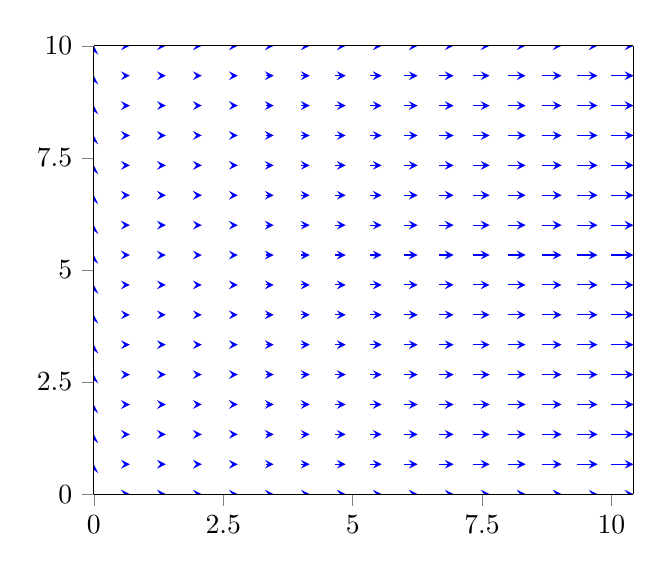
\begin{tikzpicture}
      \begin{axis}[
          view     = {0}{90}, % for a view 'from above'
          domain   = 0:10,
          y domain = 0:10,
          xtick    = {0.0, 2.5, 5.0, 7.5, 10},
          ytick    = {0.0, 2.5, 5.0, 7.5, 10},
          ytick pos = left,
          ytick align = outside,
          xtick pos = bottom,
          xtick align = outside,
        ]
        \addplot3[blue, quiver={u=x/2, v=0,
              scale arrows=0.085,
            }, -stealth, samples=16] (x,y,0);
      \end{axis}
    \end{tikzpicture}
    \label{subfig:a}
  }\hfill
  \subfloat[]{
    % \includegraphics[width=.48\linewidth]{example-image-b}
    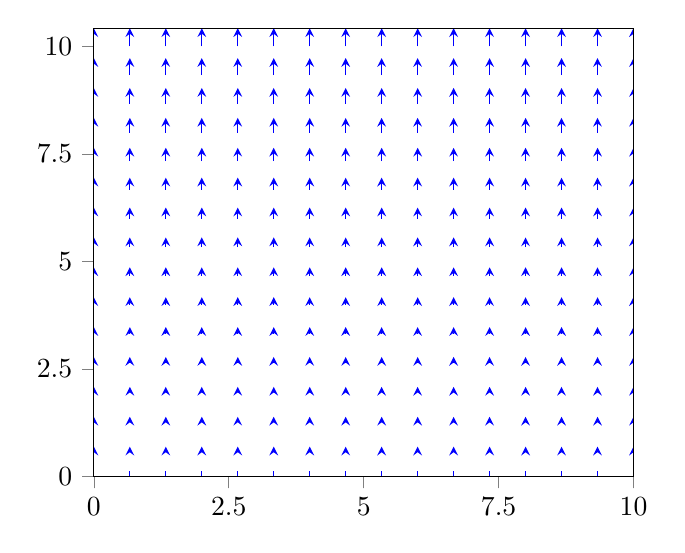
\begin{tikzpicture}
      \begin{axis}[
          view     = {0}{90}, % for a view 'from above'
          domain   = 0:10,
          y domain = 0:10,
          xtick    = {0.0, 2.5, 5.0, 7.5, 10},
          ytick    = {0.0, 2.5, 5.0, 7.5, 10},
          ytick pos = left,
          ytick align = outside,
          xtick pos = bottom,
          xtick align = outside,
        ]
        \addplot3[blue, quiver={u=0, v=y/2,
              scale arrows=0.085,
            }, -stealth, samples=16] (x,y,0);
      \end{axis}
    \end{tikzpicture}
    \label{subfig:b}
  }\\
  \subfloat[]{
    %\includegraphics[width=.48\linewidth]{example-image}
    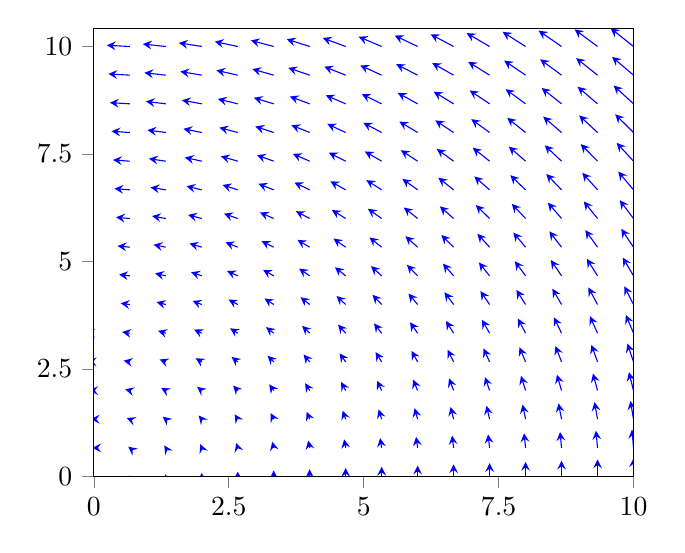
\begin{tikzpicture}
      \begin{axis}[
          view     = {0}{90}, % for a view 'from above'
          domain   = 0:10,
          xmin     = 0,
          y domain = 0:10,
          xtick    = {0.0, 2.5, 5.0, 7.5, 10},
          ytick    = {0.0, 2.5, 5.0, 7.5, 10},
          ytick pos = left,
          ytick align = outside,
          xtick pos = bottom,
          xtick align = outside,
        ]
        \addplot3[blue, quiver={u=-y/2, v=x/2,
              scale arrows=0.085,
            }, -stealth, samples=16] (x,y,0);
      \end{axis}
    \end{tikzpicture}
    \label{subfig:c}
  }\hfill
  \subfloat[]{
    %\includegraphics[width=.48\linewidth]{example-image}
    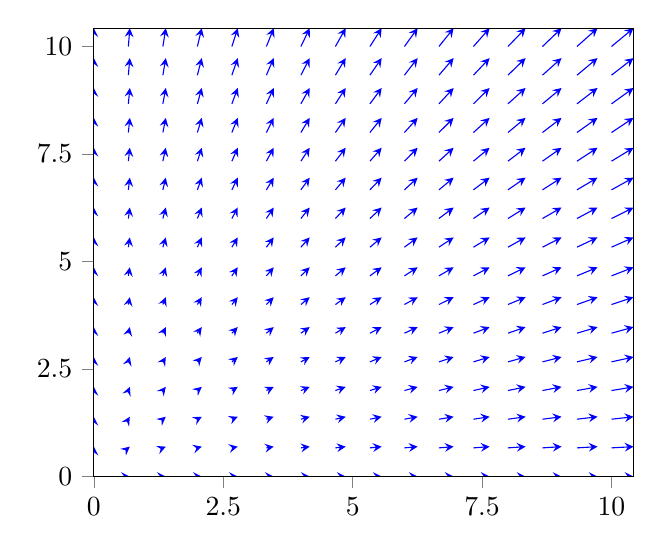
\begin{tikzpicture}
      \begin{axis}[
          view     = {0}{90}, % for a view 'from above'
          domain   = 0:10,
          y domain = 0:10,
          xtick    = {0.0, 2.5, 5.0, 7.5, 10},
          ytick    = {0.0, 2.5, 5.0, 7.5, 10},
          ytick pos = left,
          ytick align = outside,
          xtick pos = bottom,
          xtick align = outside,
        ]
        \addplot3[blue, quiver={u=x/2, v=y/2,
              scale arrows=0.085,
            }, -stealth, samples=16] (x,y,0);
      \end{axis}
    \end{tikzpicture}
    \label{subfig:d}
  }
  \caption{Plots generated with TikZ}
\end{figure*}
\end{problem}
\begin{soln}
  \begin{enumerate}[label=(\alph*)]
    \item $\mathbf{F}=x\ux+0\uy+0\uz$.
          $\Div(\mathbf{F})=\vec{\nabla} \cdot \mathbf{F}=1$.
          \begin{align*}
            \Curl(\mathbf{F}) & =\vec{\nabla} \cross \mathbf{F}                                                          \\
                              & =\begin{vmatrix}
                                   \ux                         & \uy                         & \uz                         \\
                                   \frac{\partial}{\partial x} & \frac{\partial}{\partial y} & \frac{\partial}{\partial z} \\
                                   x                           & 0                           & 0
                                 \end{vmatrix} \\
                              & = 0\ux + 0\uy+0\uz
          \end{align*}
    \item $\mathbf{F}=0\ux+y\uy+0\uz$. $\Div(\mathbf{F})=\vec{\nabla} \cdot \mathbf{F}=1$
          \begin{align*}
            \Curl(\mathbf{F}) & =\vec{\nabla} \cross \mathbf{F}                                                          \\
                              & =\begin{vmatrix}
                                   \ux                         & \uy                         & \uz                         \\
                                   \frac{\partial}{\partial x} & \frac{\partial}{\partial y} & \frac{\partial}{\partial z} \\
                                   0                           & y                           & 0
                                 \end{vmatrix} \\
                              & = 0\ux + 0\uy+ 0\uz
          \end{align*}
    \item $\mathbf{F}=-y\ux+x\uy+0\uz$. $\Div(\mathbf{F})=\vec{\nabla} \cdot \mathbf{F}=0$
          \begin{align*}
            \Curl(\mathbf{F}) & =\vec{\nabla} \cross \mathbf{F}                                                           \\
                              & =\begin{vmatrix}
                                   \ux                          & \uy                         & \uz                         \\
                                   \frac{\partial}{\partial x} & \frac{\partial}{\partial y} & \frac{\partial}{\partial z} \\
                                   -y                           & x                           & 0
                                 \end{vmatrix} \\
                              & = 0\ux + 0\uy +2\uz
          \end{align*}
    \item $\mathbf{F}=x\ux+y\uy+0\uz$. $\Div(\mathbf{F})=\vec{\nabla} \cdot \mathbf{F}=2$
          \begin{align*}
            \Curl(\mathbf{F}) & =\vec{\nabla} \cross \mathbf{F}                                                          \\
                              & =\begin{vmatrix}
                                   \ux                         & \uy                         & \uz                         \\
                                   \frac{\partial}{\partial x} & \frac{\partial}{\partial y} & \frac{\partial}{\partial z} \\
                                   -y                          & x                           & 0
                                 \end{vmatrix} \\
                              & = 0\ux + 0\uy +0\uz
          \end{align*}
  \end{enumerate}
\end{soln}
\newpage

% PROBLEM 3
\begin{problem}
Find the electric field a distance $z$ above the centre of a flat circular disk of radius $R$ that carries a uniform
charge density $\sigma$. Complete all the steps we discussed in class:
\begin{enumerate}[label=(\alph*)]
  \item State which equation you will use and draw a diagram that illustrates the variables used in the equation.
  \item Find expressions for each of the variables ($\mathbf{r}$, $\mathbf{r}^\prime$, etc.) that are needed to evaluate the equation for the field.
  \item Solve the equation for the field.
        \begin{enumerate}[label=\textbullet]
          \item Be careful to distinguish between $z > 0$ and $z < 0$.
          \item Check that your answer satisfies the boundary conditions given by Eq. (2.33) in Griffiths.
        \end{enumerate}
  \item Check that your answer makes sense in the limit $z \gg R$, where it should look like a point charge.
\end{enumerate}
\end{problem}
\begin{soln}~
  \begin{enumerate}[label=(\alph*)]
    \item For this we will use the surface charge equation,
          $$\mathbf{E}(\mathbf{r})=\frac{1}{4\pi\epsilon_0}\int\frac{\sigma(\mathbf{\primed{r}})}{\scriptr^2}\hat{\bscriptr}d\primed{a}.$$ We will integrate over the
          disk which will probably require a change to polar coordinates but means that $\primed{a}$ represents the area of the circle.
          \begin{center}
            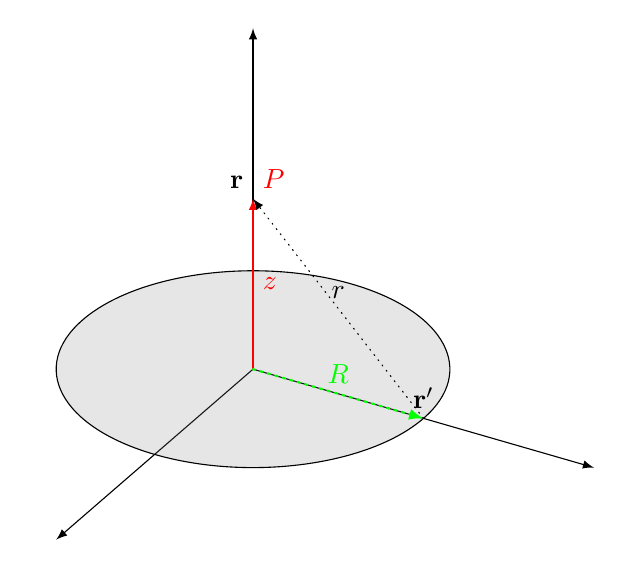
\begin{tikzpicture}[line cap=round, line join=round, scale=5, 3d view={120}{30}]
              \newcommand{\mycircle}[3] % vector x, y, z
              {%
                \pgfmathsetmacro\vtheta{atan2(#2,#1)}                     % spherical coordinate theta
                \pgfmathsetmacro\vphi  {acos(#3/sqrt(#1*#1+#2*#2+#3*#3))} % spherical coordinate phi
                \begin{scope}[rotate around z=\vtheta, rotate around y=\vphi, canvas is xy plane at z=0]
                  \draw[fill=gray,fill opacity=0.2] (0,0) circle (0.5);   % the plane, probably not needed
                \end{scope}
              }

              \draw[-latex] (0,0,0) -- (1,0,0);
              \draw[-latex] (0,0,0) -- (0,1,0);
              \draw[-latex] (0,0,0) -- (0,0,1);


              \mycircle{0}{0}{1}

              \draw[-latex,red] (0,0,0) -- (0,0,1/2) node[above right]{$P$} node[midway, right]{$z$};
              \draw[-latex, dotted, green, thick] (0,0,0) -- (0,1/2,0) node[midway, above]{$R$};
              \draw[-latex, dotted] (0,1/2,0)node[above]{$\mathbf{\primed{r}}$} -- (0,0,1/2) node[above left]{$\mathbf{r}$} node[midway, above]{$\bscriptr$};
            \end{tikzpicture}
          \end{center}
    \item $r$ is the vector to the field ``test point'', labeled $P$ in the figure. It's fairly obvious that it is $(0,0,z)$.
          $\primed{r}$ is also fairly obviously $(x,y,0)$ as it is every point s.t. $x^2+y^2\leq R^2$ (this is also our bound of integration until we make a change to polar coordinates).
          This means that $\bscriptr=(-x,-y,z)$
    \item \begin{align*}
             & = \frac{1}{4\pi\epsilon_0}\int\frac{\sigma(\mathbf{\primed{r}})}{\scriptr^2}\hat{\bscriptr}d\primed{a}                                                                                                                               \\
             & = \frac{\sigma}{4\pi\epsilon_0}\int\frac{\bscriptr}{\scriptr^3}d\primed{a}                                                                                                                                                           \\
             & = \frac{\sigma}{4\pi\epsilon_0}\int\frac{(-x,-y,z)}{\left(x^2+y^2+z^2\right)^{3/2}}d\primed{a}                                                                                                                                       \\
             & = \frac{\sigma}{4\pi\epsilon_0}\int\frac{(-x,-y,z)}{\left(x^2+y^2+z^2\right)^{3/2}}d\primed{a} \rightsquigarrow x=\primed{r}\cos\theta,y=\primed{r}\sin\theta                                                                        \\
             & = \frac{\sigma}{4\pi\epsilon_0}\int_0^{2\pi}\int_0^R\frac{(-r\cos\theta,-r\sin\theta,z)}{\left({\primed{r}}^2\cos^2\theta+{\primed{r}}^2\sin^2\theta+z^2\right)^{3/2}}\primed{r}d\primed{r}d\theta
            \rightsquigarrow x=\primed{r}\cos\theta,y=\primed{r}\sin\theta                                                                                                                                                                          \\
             & = \frac{\sigma}{4\pi\epsilon_0}\int_0^{2\pi}\int_0^R\frac{(-r\cos\theta,-r\sin\theta,z)}{\left({\primed{r}}^2+z^2\right)^{3/2}}\primed{r}d\primed{r}d\theta \quad \text{Integrating w.r.t \theta\,kills the sin and cos by symmetry} \\
             & = \frac{\sigma}{4\pi\epsilon_0}\int_{0=\primed{r}}^R\frac{(0,0,2\pi z)}{2u^{3/2}}du\rightsquigarrow u={\primed{r}}^2+z^2\implies du/2\primed{r}=d\primed{r}                                                                          \\
             & = \frac{\sigma}{4\epsilon_0}\int_{0=\primed{r}}^R\frac{(0,0,z)}{u^{3/2}}du                                                                                                                                                           \\
             & = -\frac{z\sigma}{2\epsilon_0}{\left[\left({\primed{r}}^2+z^2\right)^{-1/2}\right]}_{0}^{R}\uz=\frac{z\sigma}{2\epsilon_0}\left[\frac{1}{\abs{z}}-\frac{1}{\sqrt{R^2+z^2}}\right]\uz                                                 \\
          \end{align*}
          For boundary conditions \todo[inline]{Why do I have to discard the abs}
          \begin{align*}
            \mathbf{E}_{above}-\mathbf{E}_{below} & = \frac{z\sigma}{2\epsilon_0}\left[\frac{1}{z}-\frac{1}{\sqrt{R^2+z^2}}+\frac{1}{z}+\frac{1}{\sqrt{R^2+z^2}}\right]\uz \\
                                                  & = \frac{z\sigma}{2\epsilon_0}\left[\frac{2}{z}\right]\uz                                                               \\
                                                  & = \frac{\sigma}{\epsilon_0}\uz                                                                                         \\
          \end{align*}
          Which satisfies equation 2.33 as $\uz$ here is our normal vector.
    \item We first begin with some reworking using the binomial approximation given by $(1+x)^n\approx 1+xn$
          \begin{align*}
             & =\frac{z\sigma}{2\epsilon_0}\left[\frac{1}{z}-\frac{1}{\sqrt{R^2+z^2}}\right]\uz                \\
             & =\frac{\sigma}{2\epsilon_0}\left[1-1-\left[1+\left(\frac{R}{z}\right)^2\right]^{-1/2}\right]\uz \\
             & \approx\frac{\sigma}{2\epsilon_0}\left[\frac{R^2}{2z^2}\right] \uz                              \\
             & =\frac{\sigma R^2}{4\epsilon_0z^2}\uz
          \end{align*}
          We then recognize that $\sigma=Q/\pi R^2$ because we have a uniform charge distribution of net charge $Q$ spread over a disk of area $\pi R^2$.
          Substituting this in,
          $$
            \frac{QR^2}{4\epsilon_0\pi R^2z^2}\uz=\frac{Q}{4\pi\epsilon_0 z^2}\uz
          $$
          Which is the equation for a point charge, as we would hope.
  \end{enumerate}
\end{soln}

% PROBLEM 4
\begin{problem}
For a solid sphere of radius $R$ and charge density $\rho(\mathbf{r}) = \kappa r$, use Gauss' law to find
\begin{enumerate}[label=(\roman*)]
  \item The electric field.
  \item The potential inside and outside the sphere.
\end{enumerate}
\end{problem}
\begin{soln}~
  \begin{enumerate}[label=(\roman*)]
    \item Gauss' law states that
          $$\oint_S \mathbf{E}\cdot d\mathbf{a}=\frac{Q_{enc}}{\epsilon_0}$$
          Where $Q_{enc}$ is given by
          $$Q_{enc}=\int_\mathcal{V}\rho \,d\tau.$$
          Because we have a sphere of charge we can transform this to use spherical coordinates,
          \begin{align*}
            Q_{enc} & =\int_0^R dr \int_0^{\pi} d\theta \int_0^{2\pi}d\phi\,kr^3\sin\theta \\
                    & =4\pi k\int_0^R r^3 dr                                               \\
                    & =\pi kR^4
          \end{align*}
          We can now return to our original statement involving $\mathbf{E}$ and solve. We can also observe that because
          $\mathbf{E}$ points radially outwards from our sphere and $\mathbf{a}$ does as well we can reduce the dot product to a product of their magnitudes.
          $$
            \frac{\pi kR^4}{\epsilon_0}= \oint_S \abs{\mathbf{E}} da
          $$
          Now because $\abs{\mathbf{E}}$ is constant over the \emph{surface} because the charge density is spherically symmetric, only depending on $r$,
          we can extract $\abs{\mathbf{E}}$ from the integral which then just becomes the area of a sphere,
          \begin{align*}
            \frac{\pi kR^4}{\epsilon_0}  & = \oint_S \abs{\mathbf{E}} da  \\
            \frac{\pi kR^4}{\epsilon_0}  & = \abs{\mathbf{E}} \oint_S  da \\
            \frac{\pi kR^4}{\epsilon_0}  & = 4\pi r^2 \abs{\mathbf{E}}    \\
            \frac{kR^4}{4\epsilon_0 r^2} & = \abs{\mathbf{E}}             \\
          \end{align*}
          (For $r>R$)
    \item To start here we need the electric field inside the sphere which is given by the same process as above except we integrate from $0$ to $r\leq R$
          because we are now inside the sphere. This gives $Q_enc=\pi kr^4\implies \mathbf{E}=\frac{kr^2}{4\epsilon_0}\hat{\mathbf{r}}$. We can now evaluate for the outside of the sphere,
          \begin{align*}
            V_{r>R}(r) & =-\int_\infty^r\frac{kR^4}{4\epsilon_0 {\primed{r}}^2}d\primed{r}                             \\
                       & =-\int_\infty^r\frac{kR^4}{4\epsilon_0 {\primed{r}}^2}d\primed{r}                             \\
                       & =\frac{kR^4}{4\epsilon_0}\left[\frac{1}{\primed{r}}\right]_\infty^r=\frac{kR^4}{4\epsilon_0r}
          \end{align*}
          Then for the potential inside the sphere we split the integral. \todo[inline]{I'm not sure why we do this but it's done in the text}
          \begin{align*}
            V_{R<r}(r) & =-\int_\infty^R\frac{kR^4}{4\epsilon_0 {\primed{r}}^2}d\primed{r}-\int_R^r\frac{kr^2}{4\epsilon_0}d\primed{r} \\
                       & =\frac{kR^4}{4\epsilon_0R}-\frac{k}{12\epsilon_0}\left[{\primed{r}}^3\right]_R^r                              \\
                       & =\frac{k}{12\epsilon_0}\left(4R^3-r^3\right)
          \end{align*}
          \todo[inline]{Check both of these w/ $E=-\nabla V$}
  \end{enumerate}
\end{soln}

% PROBLEM 5
\begin{problem}
Consider the electric field
$$\mathbf{E}(\mathbf{r})=E_0\left[y^2\ux+\left(2xy+z^2\right)\uy+2yz\uz\right].$$
Find, by integrating $-\int\mathbf{E}\cdot d\boldsymbol{\ell}$, the potential at an arbitrary point $\mathbf{r}$, taking the origin as the reference point.
Note that the most direct integration path may not be simplest.
\end{problem}
\begin{soln}
  Here we have that $d\boldsymbol{\ell}=dx\ux+dy\uy+dz\uz$ which means that
  $\mathbf{E}\cdot d\boldsymbol{\ell}=E_0\left[y^2dx+\left(2xy+z^2\right)dy+2yzdz\right]$ so,
  \begin{align*}
     & V(\mathbf{r})= -\int_0^{\mathbf{r}}E_0\left[y^2dx+\left(2xy+z^2\right)dy+2yzdz\right]     \\
     & = -E_0\left[\int_0^{r_x}y^2dx+\int_0^{r_y}\left(2xy+z^2\right)dy+\int_0^{r_z}2yzdz\right]
  \end{align*}
  Which simplifies nicely along several paths (though it's already fairly simple). I'll go along the $x$, the $y$, then the $z$.
  This means that for our first integral along $x$ we are moving from $\langle0,0,0\rangle$ to $\langle r_x,0,0\rangle$ so $y$ is zero
  along the whole range which means that the integral just becomes zero as its integrand is $y^2$. Next along
  $y$ we are moving from $\langle r_x,0,0\rangle$ to $\langle r_x,r_y,0\rangle$ so
  $$\int_0^{r_y}\left(2xy+\cancelto{0}{z^2}\right)dy=r_xr_y^2.$$
  Finally along $z$ we are moving from $\langle r_x,r_y,0\rangle$ to $\langle r_x,r_y,r_z\rangle$ so
  $$\int_0^{r_z}2yzdz=\int_0^{r_z}2yzdz=r_yr_z^2.$$
  This yields
  $$V(\mathbf{r})=-E_0\left[r_xr_y^2 + r_yr_z^2\right].$$
\end{soln}
\end{document}